\documentclass[t,dvipsnames,table]{beamer}
\usetheme{Copenhagen}
\setbeamertemplate{headline}{} % remove toc from headers
\beamertemplatenavigationsymbolsempty

\usepackage{amsmath, array, tikz, xcolor, tcolorbox, bm, tkz-euclide, pgfplots, graphicx}
\pgfplotsset{compat = 1.16}
\usetkzobj{all}
\everymath{\displaystyle}

\title{Hyperbolas}
\author{}
\date{}

\AtBeginSection[]
{
  \begin{frame}
    \frametitle{Objectives}
    \tableofcontents[currentsection]
  \end{frame}
}

\begin{document}

\begin{frame} 
\maketitle
\end{frame}

\begin{frame}[c]
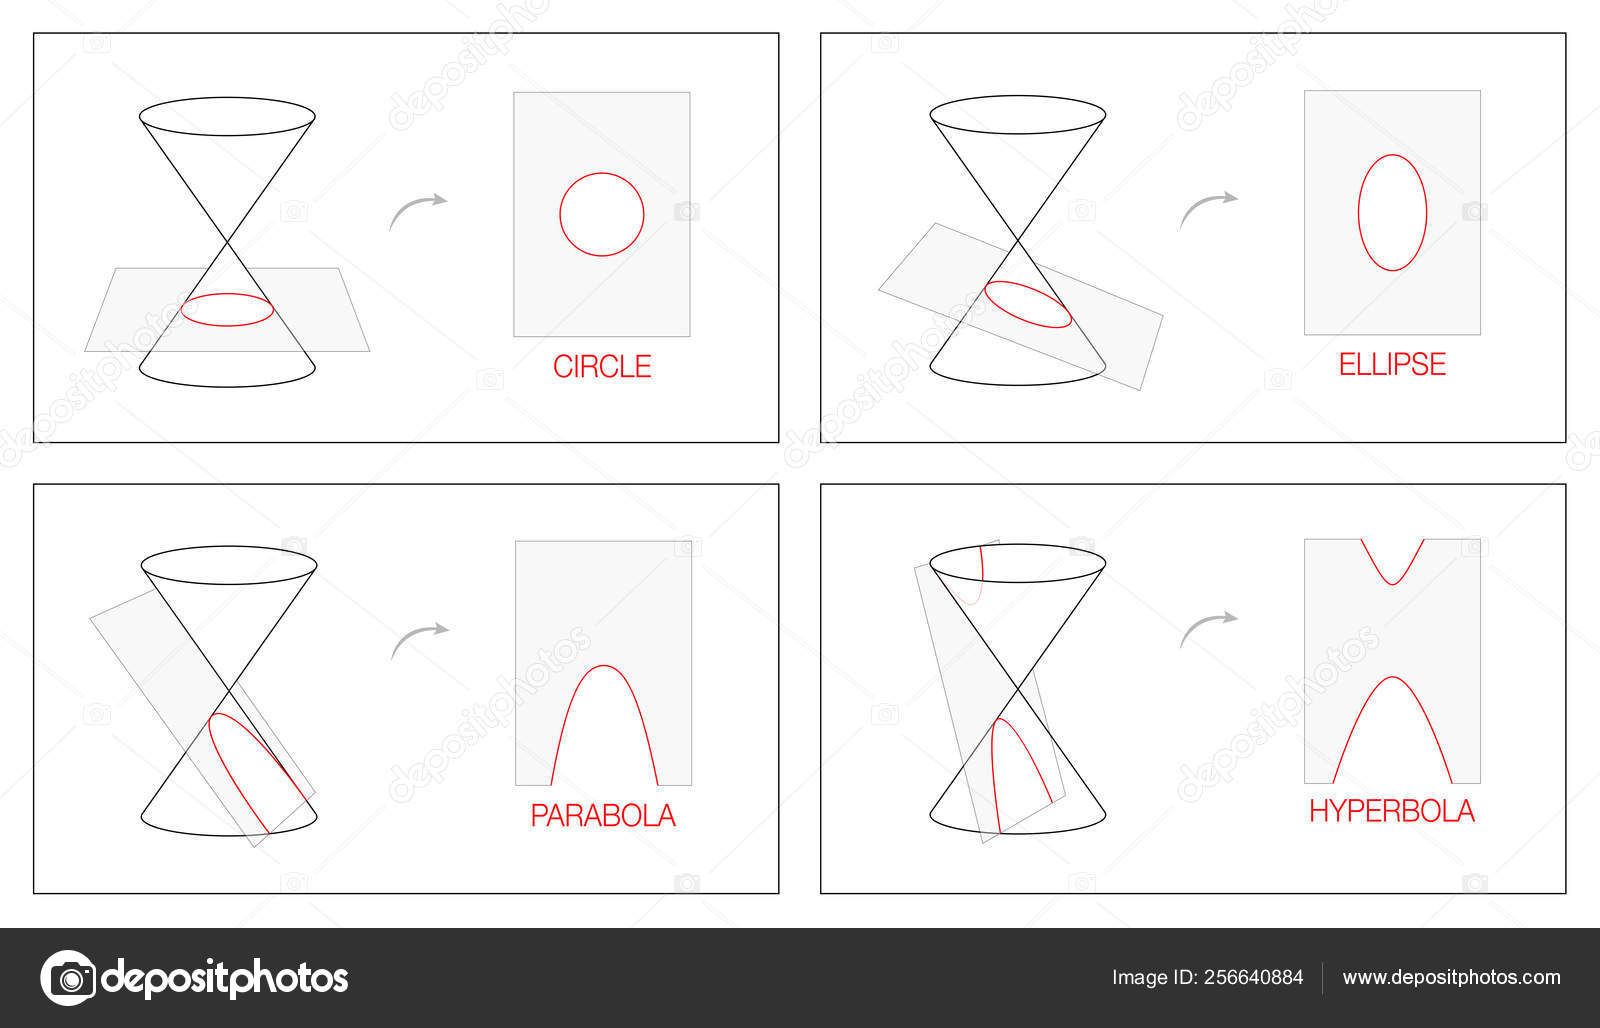
\includegraphics[scale=0.80]{Images/conics.jpg}
\end{frame}

\section{Find the vertices and foci for a hyperbola in standard form.}

\begin{frame}{Hyperbolas}
\begin{tcolorbox}[colback=red!10!white, colframe=red!60!black,, title=\textbf{Hyperbolas}]
The set of points such that the \textbf{difference} of their distances from 2 fixed points (called \textbf{foci}) is constant.
\end{tcolorbox}
\vspace{11pt}	\pause
\end{frame}

\begin{frame}{Comparing Hyperbolas and Ellipses}

Just like an ellipse, the midpoint joining the foci is the \textbf{center}.    \newline\\	\pause 

Whereas ellipses could appear taller or wider, hyperbolas will open up and down, or left and right. \newline\\ \pause 

A key difference, however, is that hyperbolas will open left/right if the sign in front of $x$ is positive, and will open up/down if the sign in front of $y$ is positive; regardless of the values of $a$ and $b$.
\end{frame}

\begin{frame}[c]{Opening Left and Right}
\begin{center}
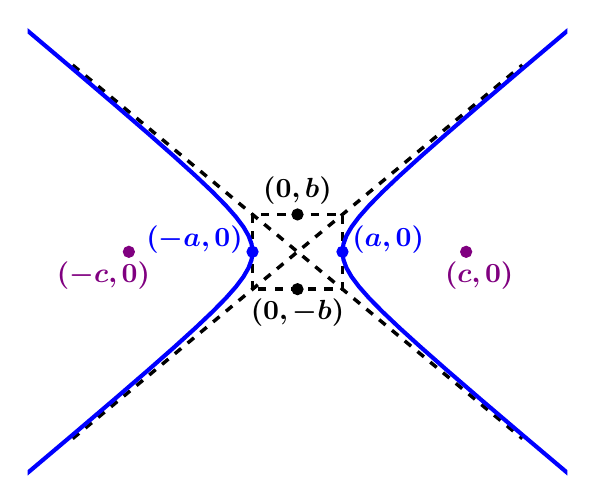
\begin{tikzpicture}
\begin{axis}[
axis lines = none,
%grid,
xticklabels = {},
yticklabels = {},
xmin = -6, xmax = 6,
ymin = -6, ymax = 6
]
\draw [dashed, line width=1.25] (-1,-1) rectangle (1,1);
\draw [dashed, line width=1.25] (-5,-5) -- (5,5);
\draw [dashed, line width=1.25] (-5,5) -- (5,-5);
\addplot [blue, line width = 1.5, domain=-2.5:2.5] ({cosh(x)}, {sinh(x)});
\addplot [blue, line width = 1.5, domain=-2.5:2.5] (-{cosh(x)}, {sinh(x)});
\draw [fill=blue, color=blue] (-1,0) circle (2pt);
\node at (-1,0) [anchor=south east, color=blue, yshift=-0.15cm] {$\bm{(-a,0)}$};
\draw [fill=blue, color=blue] (1,0) circle (2pt);
\node at (1,0) [anchor=south west, color=blue, yshift=-0.15cm] {$\bm{(a,0)}$};
\draw [fill=violet, color=violet] (3.75,0) circle (2pt);
\node at (3.5,0) [anchor=north west, color=violet, xshift=-0.25cm] {$\bm{(c,0)}$};
\draw [fill=violet, color=violet] (-3.75,0) circle (2pt);
\node at (-3.5,0) [anchor=north east, color=violet, xshift=0.25cm] {$\bm{(-c,0)}$};
\draw [fill=black] (0,1) circle (2pt);
\node at (0,1) [anchor=south] {$\bm{(0,b)}$};
\draw [fill=black] (0,-1) circle (2pt);
\node at (0,-1) [anchor=north] {$\bm{(0,-b)}$};
\end{axis}
\end{tikzpicture}
\end{center}
\end{frame}

\begin{frame}{Properties}
\begin{tabular}{cc}
    \textbf{Equation}  &   $\dfrac{(x-h)^2}{a^2} - \dfrac{(y-k)^2}{b^2} = 1$   \\[15pt]
    \textbf{Center}		&	$(h,k)$	\\[11pt]
    \textbf{Vertices}   &   $(h\pm a,0)$ \\[11pt]
    \textbf{Foci}   &   $(h\pm c,0)$   \\[11pt]
    \textbf{Co-vertices} & $(h, k \pm b)$	\\[11pt]
    \textbf{\textit{x}-Axis}    &   Transverse Axis     \\[11pt]
    \textbf{\textit{y}-Axis}    &   Conjugate Axis      \\[111pt]
    $\bm{c^2}$  &   $a^2+b^2$  \\    
\end{tabular}
\end{frame}

\begin{frame}[c]{Opening Up and Down}
\begin{center}
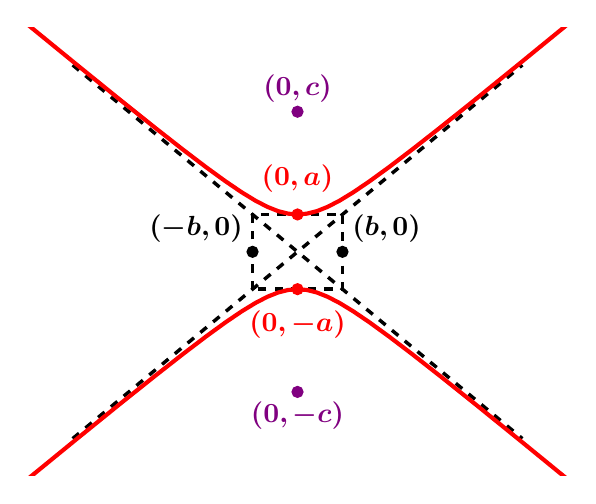
\begin{tikzpicture}
\begin{axis}[
axis lines = none,
%grid,
xticklabels = {},
yticklabels = {},
xmin = -6, xmax = 6,
ymin = -6, ymax = 6
]
\draw [dashed, line width=1.25] (-1,-1) rectangle (1,1);
\draw [dashed, line width=1.25] (-5,-5) -- (5,5);
\draw [dashed, line width=1.25] (-5,5) -- (5,-5);
\addplot [red, line width = 1.5, domain=-2.5:2.5] ({sinh(x)}, {cosh(x)});
\addplot [red, line width = 1.5, domain=-2.5:2.5] ({sinh(x)}, {-cosh(x)});
\draw [fill=red, color=red] (0,1) circle (2pt);
\node at (0,1) [anchor=south, color=red, yshift=0.15cm] {$\bm{(0,a)}$};
\draw [fill=blue, color=red] (0,-1) circle (2pt);
\node at (0,-1) [anchor=north, color=red, yshift=-0.15cm] {$\bm{(0,-a)}$};
\draw [fill=violet, color=violet] (0,3.75) circle (2pt);
\node at (0,3.75) [anchor=south, color=violet] {$\bm{(0,c)}$};
\draw [fill=violet, color=violet] (0,-3.75) circle (2pt);
\node at (0,-3.75) [anchor=north, color=violet] {$\bm{(0,-c)}$};
\draw [fill=black] (1,0) circle (2pt);
\node at (1,0) [anchor=south west] {$\bm{(b,0)}$};
\draw [fill=black] (-1,0) circle (2pt);
\node at (-1,0) [anchor=south east] {$\bm{(-b,0)}$};
\end{axis}
\end{tikzpicture}
\end{center}
\end{frame}

\begin{frame}{Properties}
\begin{tabular}{cc}
    \textbf{Equation}  &   $\dfrac{(y-k)^2}{a^2} - \dfrac{(x-h)^2}{b^2} = 1$   \\[15pt]
    \textbf{Center}		&	$(h,k)$	\\[11pt]
    \textbf{Vertices}   &   $(h, k\pm a)$ \\[11pt]
    \textbf{Foci}   &   $(h, k \pm c)$   \\[11pt]
    \textbf{Co-vertices} & $(h \pm a, k)$	\\[11pt]
    \textbf{\textit{x}-Axis}    &   Conjugate Axis     \\[11pt]
    \textbf{\textit{y}-Axis}    &   Transverse Axis      \\[111pt]
    $\bm{c^2}$  &   $a^2+b^2$  \\    
\end{tabular}
\end{frame}

\begin{frame}{Example 1}
Find the exact coordinates for the vertices and foci for each of the following.	\newline\\
(a)	\quad	$\dfrac{(y-3)^2}{4} - \dfrac{x^2}{16} = 1$	\newline\\
\onslide<2->{Center: $(0,3)$}	\newline\\
\onslide<3->{$a^2 = 4$}	\newline\\
\onslide<4->{$a = \pm 2$} \newline\\
\onslide<5->{Vertices: $(0, 3 \pm 2)$} \onslide<6->{$\longrightarrow (0, 1) \text{ and } (0, 5)$}
\end{frame}

\begin{frame}{Example 1a}
\begin{align*}
c^2 &= a^2 + b^2	\\[6pt]
\onslide<2->{c^2 &= 4 + 16} \\[6pt]
\onslide<3->{c^2 &= 20}	\\[6pt]
\onslide<4->{c &= \pm 2\sqrt{5}}	\\[8pt]
\end{align*}
\onslide<5->{Foci: $(0, 3 \pm 2\sqrt{5})$}
\end{frame}


\section{Write the equation for a hyperbola in standard form.}

\end{document}